\section{Simulation Analysis}
\label{sec:simulation}



\subsection{Operating point analysis for t<0}

In this section, an operating point analysis of the circuit (referência ao circuito) was conducted in order to calculate the voltage in all nodes and the current through the resistors for a t < 0. To contextualize the values obtained using the tools in ngspice, it is necessary to state that, as node 0 is connected to ground, its nodal voltage does not appear on the table of results. It is important to note that an extra voltage source, Vaux, was added and therefore, another node was also added (node 9). This Vaux was intended to allow the measurement of the current Ic which voltage source Vc depends on, since ngspice doesn't allow us to introduce Resistor R6's current in the computation. Vaux's voltage is equal to 0 V, since it is only an auxiliary component that doesn't interfere with the circuit (node's 7 voltage is equal to node's 9 voltage) and allowed us to obtain the current through it.

\begin{table}[H] \centering
\begin{tabular}{|
>{\columncolor[HTML]{FFCC67}}l l
>{\columncolor[HTML]{FFCC67}}l l|}
\hline
\cellcolor[HTML]{EABD8B}Name & \cellcolor[HTML]{EABD8B}Value {[}A or V{]} & \cellcolor[HTML]{EABD8B}Name & \cellcolor[HTML]{EABD8B}Value {[}A or V{]} \\ \hline
@gb                          & -2.86455e-04                               & V1                           & 5.216040e+00                                   \\
@R1{[}i{]}                   & 2.732478e-04                               & V2                           & 4.939074e+00                                   \\
@R2{[}i{]}                   & -2.86455e-04                               & V3                           & 4.361415e+00                                   \\
@R3{[}i{]}                   & -1.32073e-05                               & V5                           & 4.978786e+00                                 \\
@R4{[}i{]}                   & 1.229564e-03                               & V6                           & 5.853598e+00                               \\
@R5{[}i{]}                   & 1.316042e-03                               & V7                          & 
-2.00109e+00       \\
@R6{[}i{]}                   & 9.563162e-04                               & V8                           & -2.97875e+00                               \\
@R7{[}i{]}                   & 9.563162e-04                               & V9                           & 
0.000000e+00       \\
 \hline
\end{tabular}
\caption{NgSpice simulation results 1}
\end{table}



\subsection{Calculus of $Req$ - Simulation}

Similarly to the last section, an operating point analysis to the circuit (referência ao circuito) was conducted, with the difference being that the voltage source $vs$ was turned off and the capacitor was replaced by the independent voltage source Vx which corresponds to the value of $v(6)$-$v(8)$. This Vx is equivalent to the voltage in the capacitor's terminals. 
The values of currents and nodal voltages were then put in a table, as well as the Req, hence:

\begin{table}[H] \centering
\begin{tabular}{|
>{\columncolor[HTML]{FFCC67}}l l
>{\columncolor[HTML]{FFCC67}}l l|}
\hline
\cellcolor[HTML]{EABD8B}Name & \cellcolor[HTML]{EABD8B}Value {[}A or V{]} & \cellcolor[HTML]{EABD8B}Name & \cellcolor[HTML]{EABD8B}Value {[}A or V{]} \\ \hline
@gb                          & 0.000000e+00                               & V1                           & 0.000000e+00                                  \\
@R1{[}i{]}                   & 0.000000e+00                               & V2                           & 0.000000e+00                                   \\
@R2{[}i{]}                   & 0.000000e+00                               & V3                           & 0.000000e+00                                   \\
@R3{[}i{]}                   & 0.000000e+00                               & V5                           & 0.000000e+00                                 \\
@R4{[}i{]}                   & 0.000000e+00                               & V6                           & 5.000000e+01                               \\
@R5{[}i{]}                   & -1.63724e-02                               & V7                          & 
0.000000e+00      \\
@R6{[}i{]}                   & 0.000000e+00                               & V8                           & 0.000000e+00                              \\
@R7{[}i{]}                   & 0.000000e+00                               & V9                           & 
0.000000e+00       \\
 \hline
\end{tabular}
\caption{NgSpice simulation results 2}
\end{table} 

\begin{equation}
Req = (v(6)-v(8))/vxbranch,
\end{equation}
with vxbranch corresponding to the current Ix that flows through the Vx's branch.

\subsection{Operating Point Analysis for t $\geq$ (Natural Solution)}

In this section, a transient analysis was conducted in order to evaluate the natural response of the circuit, which means, the variation over time. Once that to calculate the natural response, the voltage source $vs$ is turned off, so the circuit simulated was equal to the one in the previous question. From this, the voltage in the capacitor's over time (time interval considered was [0,20]ms) was calculated and plotted.

\begin{figure}[h] \centering

\begin{subfigure}{0.4\textwidth}
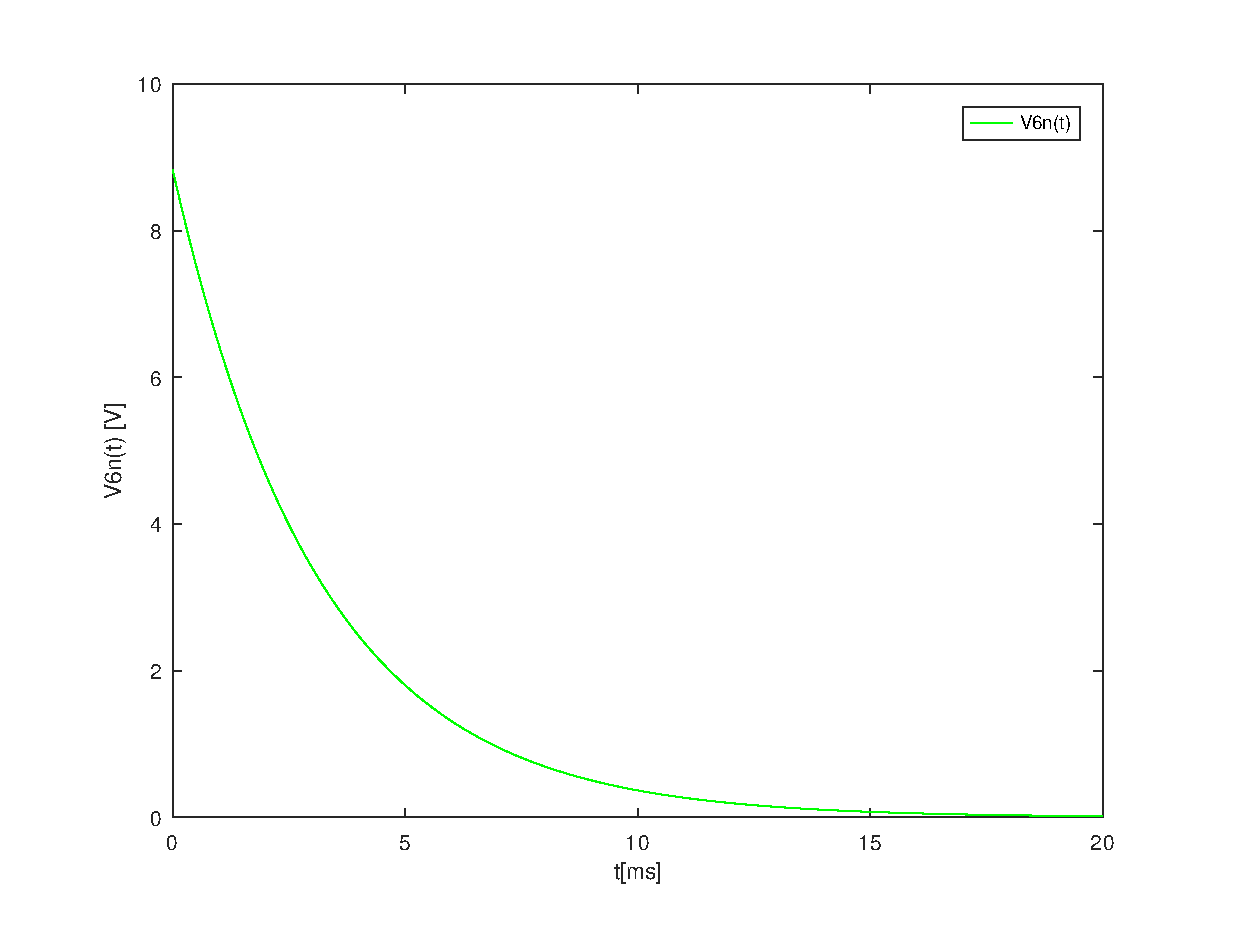
\includegraphics[width=\textwidth]{NaturalResponse.eps}
\caption{Natural Response (Octave)}
\label{fig:first}
\end{subfigure}
\begin{subfigure}{0.4\textwidth}
\includegraphics[width=\textwidth]{sim_3.pdf}
\caption{Natural Response (NGSpice)}
\label{fig:second}
\end{subfigure}

\end{figure}
 
\subsection{Operating Point Analysis for t $\geq$ (Natural and Forced Solution)}
In this section, as previously, a transient analysis was conducted in order to evaluate the natural and forced response of the circuit. In order to achieve this, the procedure adopted was the same as the one in the previous step, but with the voltage souce $vs(t)$ as sinusoidal wave %sen(2*\pi*f).  

\begin{figure}[h] \centering

\begin{subfigure}{0.4\textwidth}
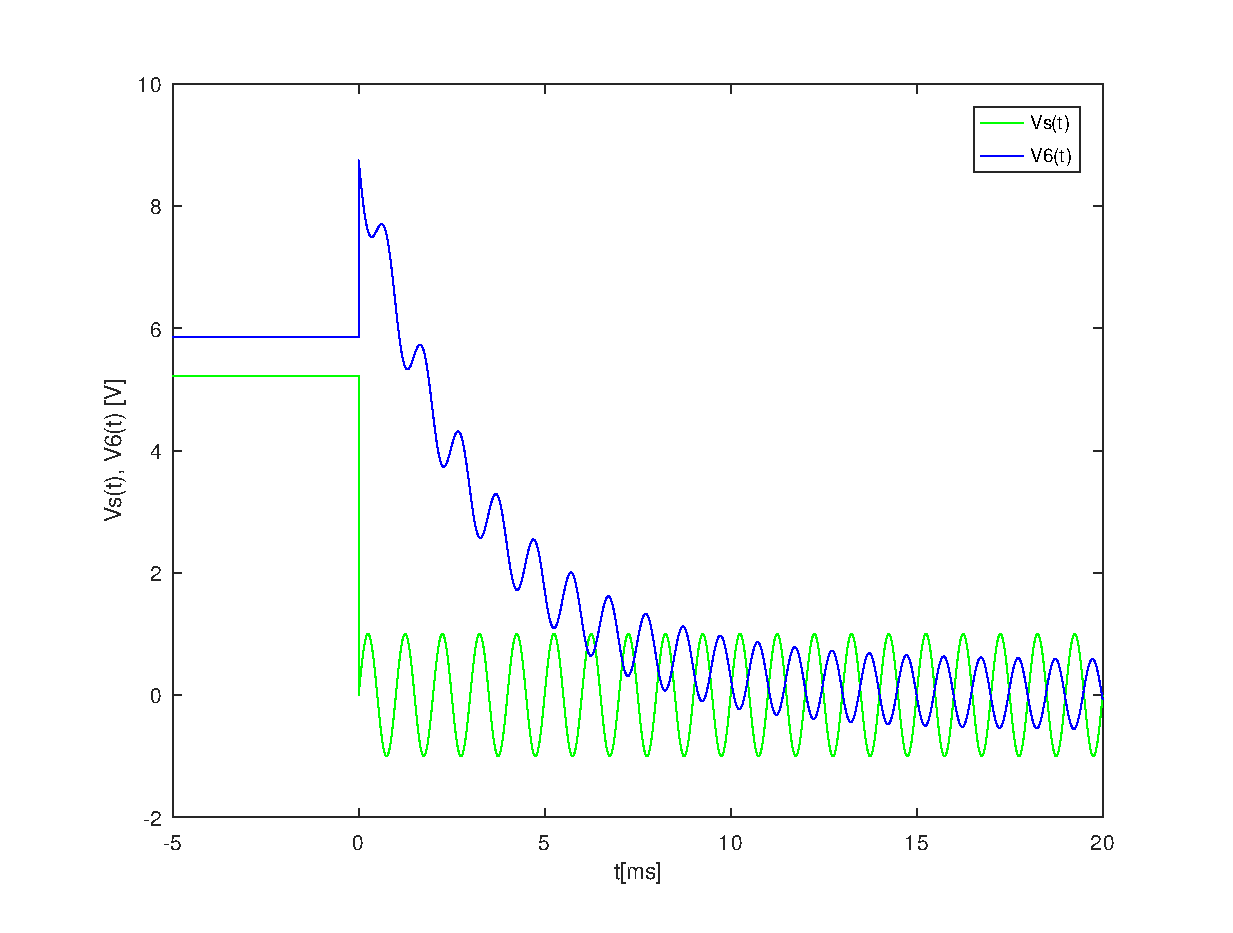
\includegraphics[width=\textwidth]{Solution.eps}
\caption{Natural and forced response (Octave)}
\label{fig:first}
\end{subfigure}
\begin{subfigure}{0.4\textwidth}
\includegraphics[width=\textwidth]{sim4.pdf}
\caption{Natural and forced response}
\label{fig:second}
\end{subfigure}

\end{figure}

\subsection{Frequency Responses}

In this part of the assignment, an AC (Small Signal Analysis was conducted, in order to match the goal afore-
mentioned. This type of analysis allows to study the frequency response of the circuit. In other words, there
is no frequency variation over time, the so called steady-state analysis.After comparing the graphics showed
below, it is clear to admit that the results in ngspice and octave match. Any minor difference may be explained
by aproximation errors.

\subsubsection{Frequency Responses - Amplitude}



\begin{figure}[h] \centering

\begin{subfigure}{0.4\textwidth}
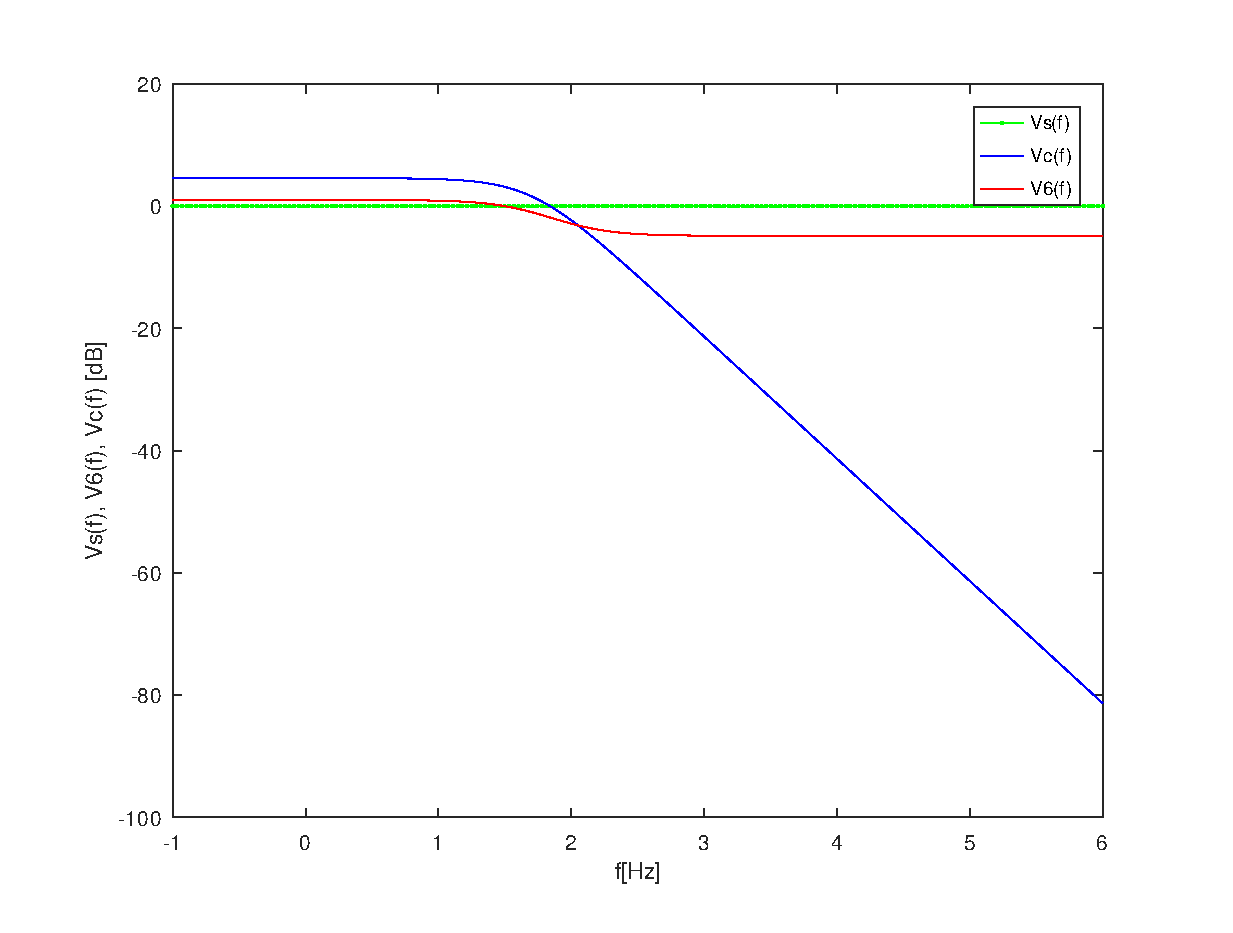
\includegraphics[width=\textwidth]{Amplitude.eps}
\caption{First Circuit}
\label{fig:first}
\end{subfigure}
\begin{subfigure}{0.4\textwidth}
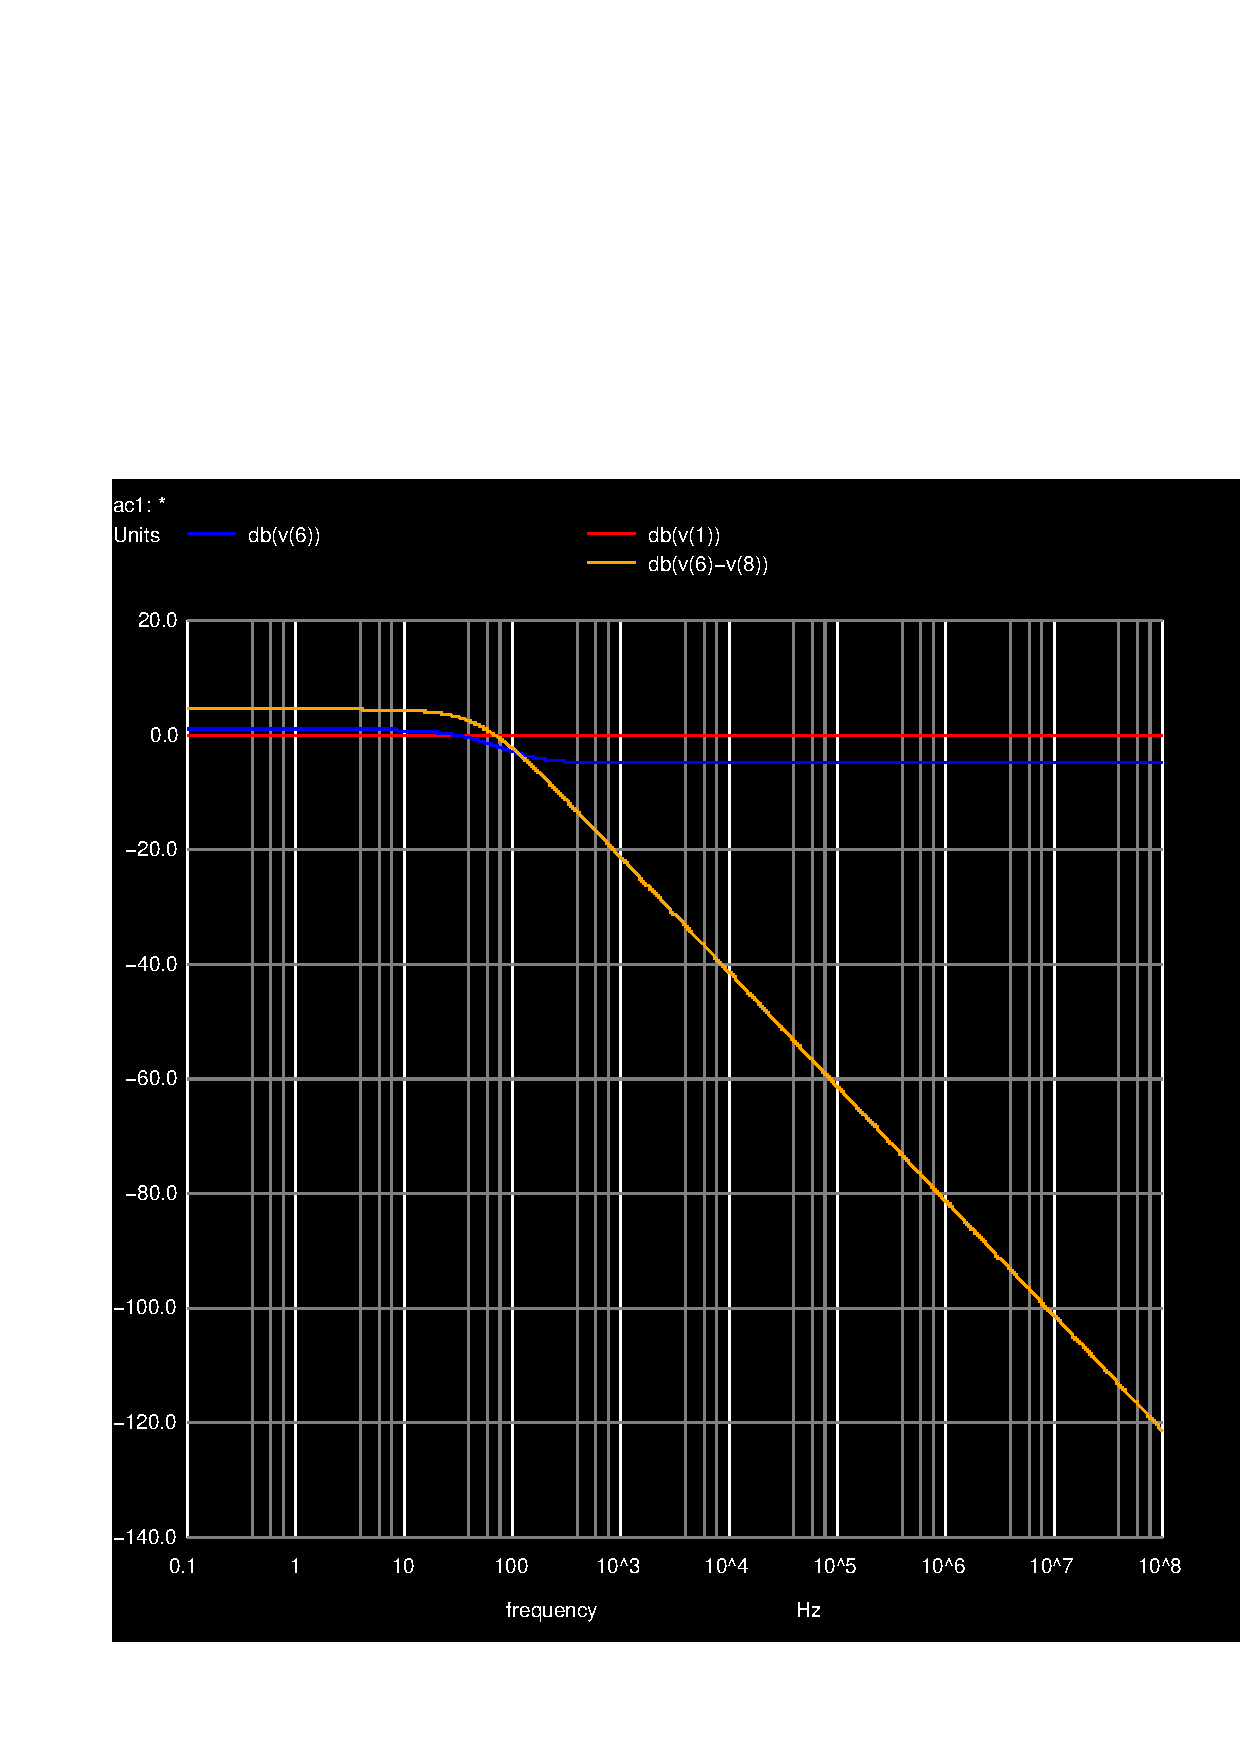
\includegraphics[width=\textwidth]{sim5_db.pdf}
\caption{Second Circuit}
\label{fig:second}
\end{subfigure}

\end{figure}

\subsubsection{Frequency Responses - Phase}

\begin{figure}[h] \centering

\begin{subfigure}{0.4\textwidth}
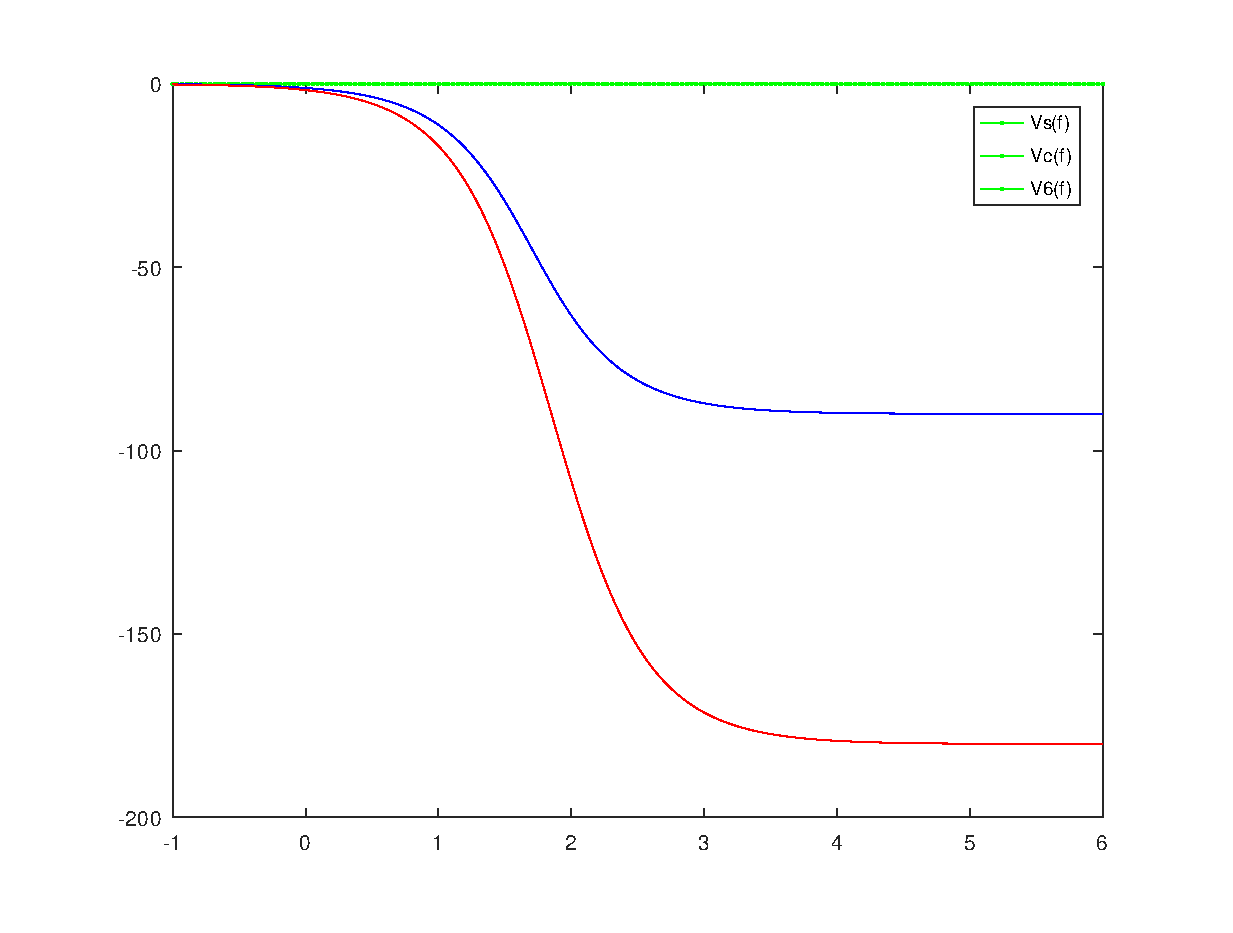
\includegraphics[width=\textwidth]{Arguments.eps}
\caption{First Circuit}
\label{fig:first}
\end{subfigure}
\begin{subfigure}{0.4\textwidth}
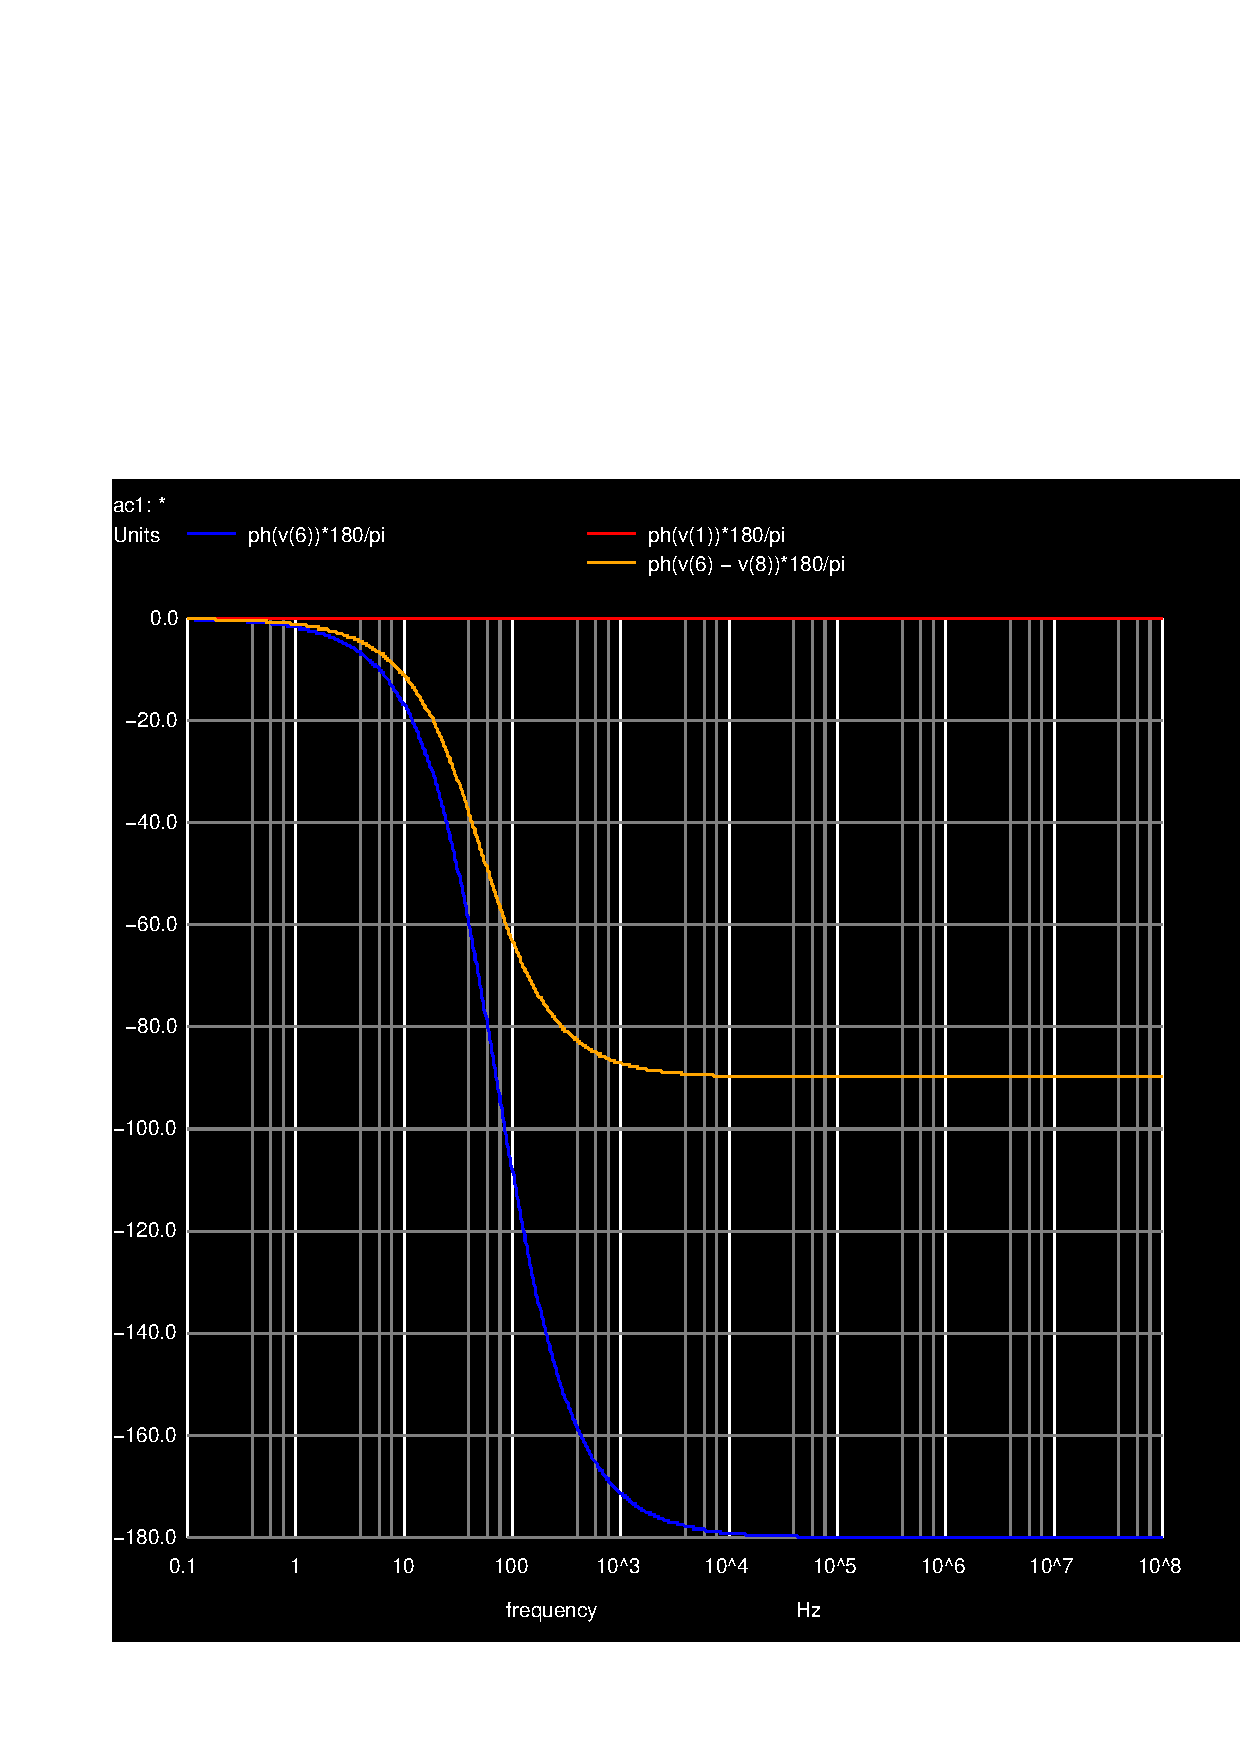
\includegraphics[width=\textwidth]{sim5_ph.pdf}
\caption{Second Circuit}
\label{fig:second}
\end{subfigure}

\end{figure}

\section{Octave and Ngspice comparisation}




%se for preciso
%\end{figure}
%\begin{figure}[H]
%\centering
%\includegraphics[width = 15cm]{sim_3.pdf}
%\caption {Ngspice simulation plot 1}
%\end{figure}



%se for preciso
%\begin{figure}[H]
%\centering
%\includegraphics[width = 15cm]{sim4.pdf}
%\caption {Ngspice simulation plot 2}
%\end{figure}




%se for preciso
%\begin{figure}[H]
%\centering
%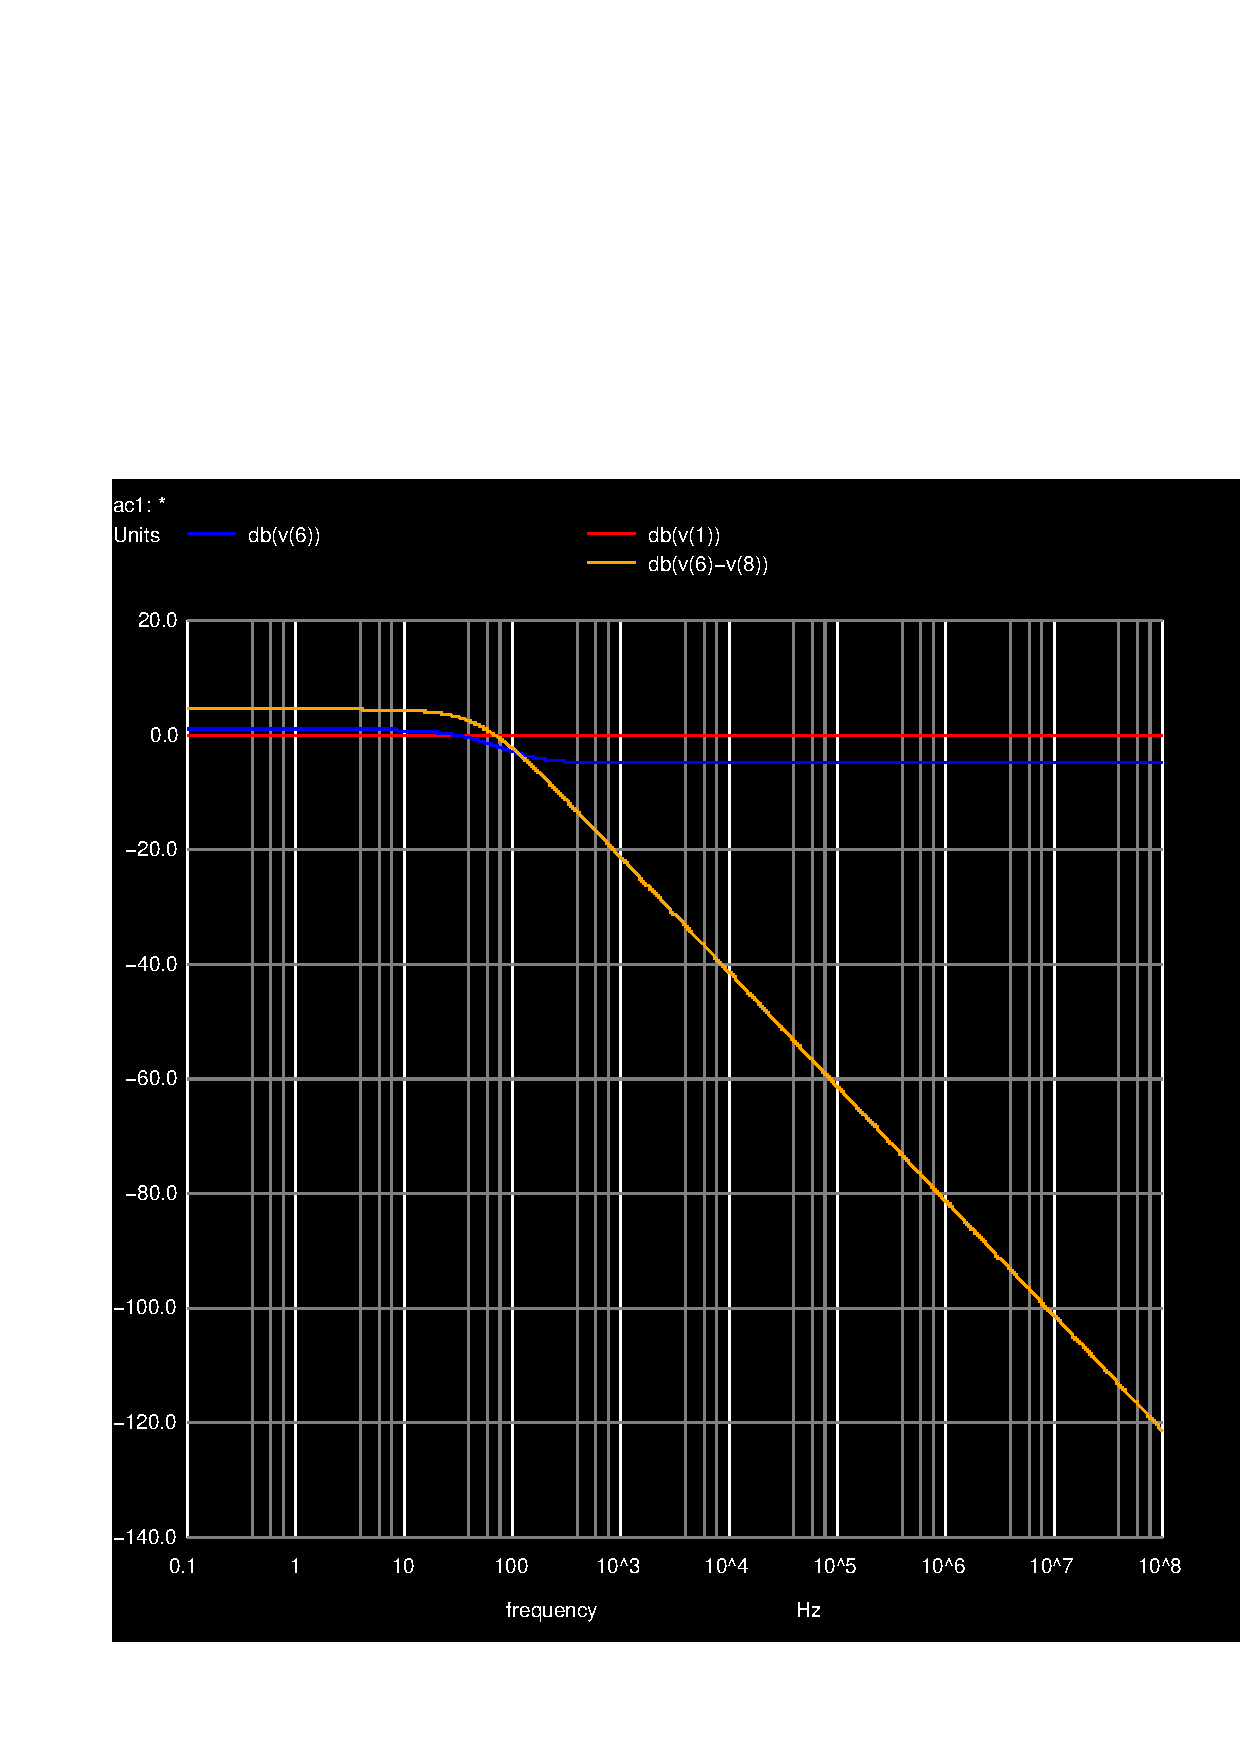
\includegraphics[width = 15cm]{sim5_db.pdf}
%\caption {Ngspice simulation plot 3}
%\end{figure}




%se for preciso
%\begin{figure}[H]
%\centering
%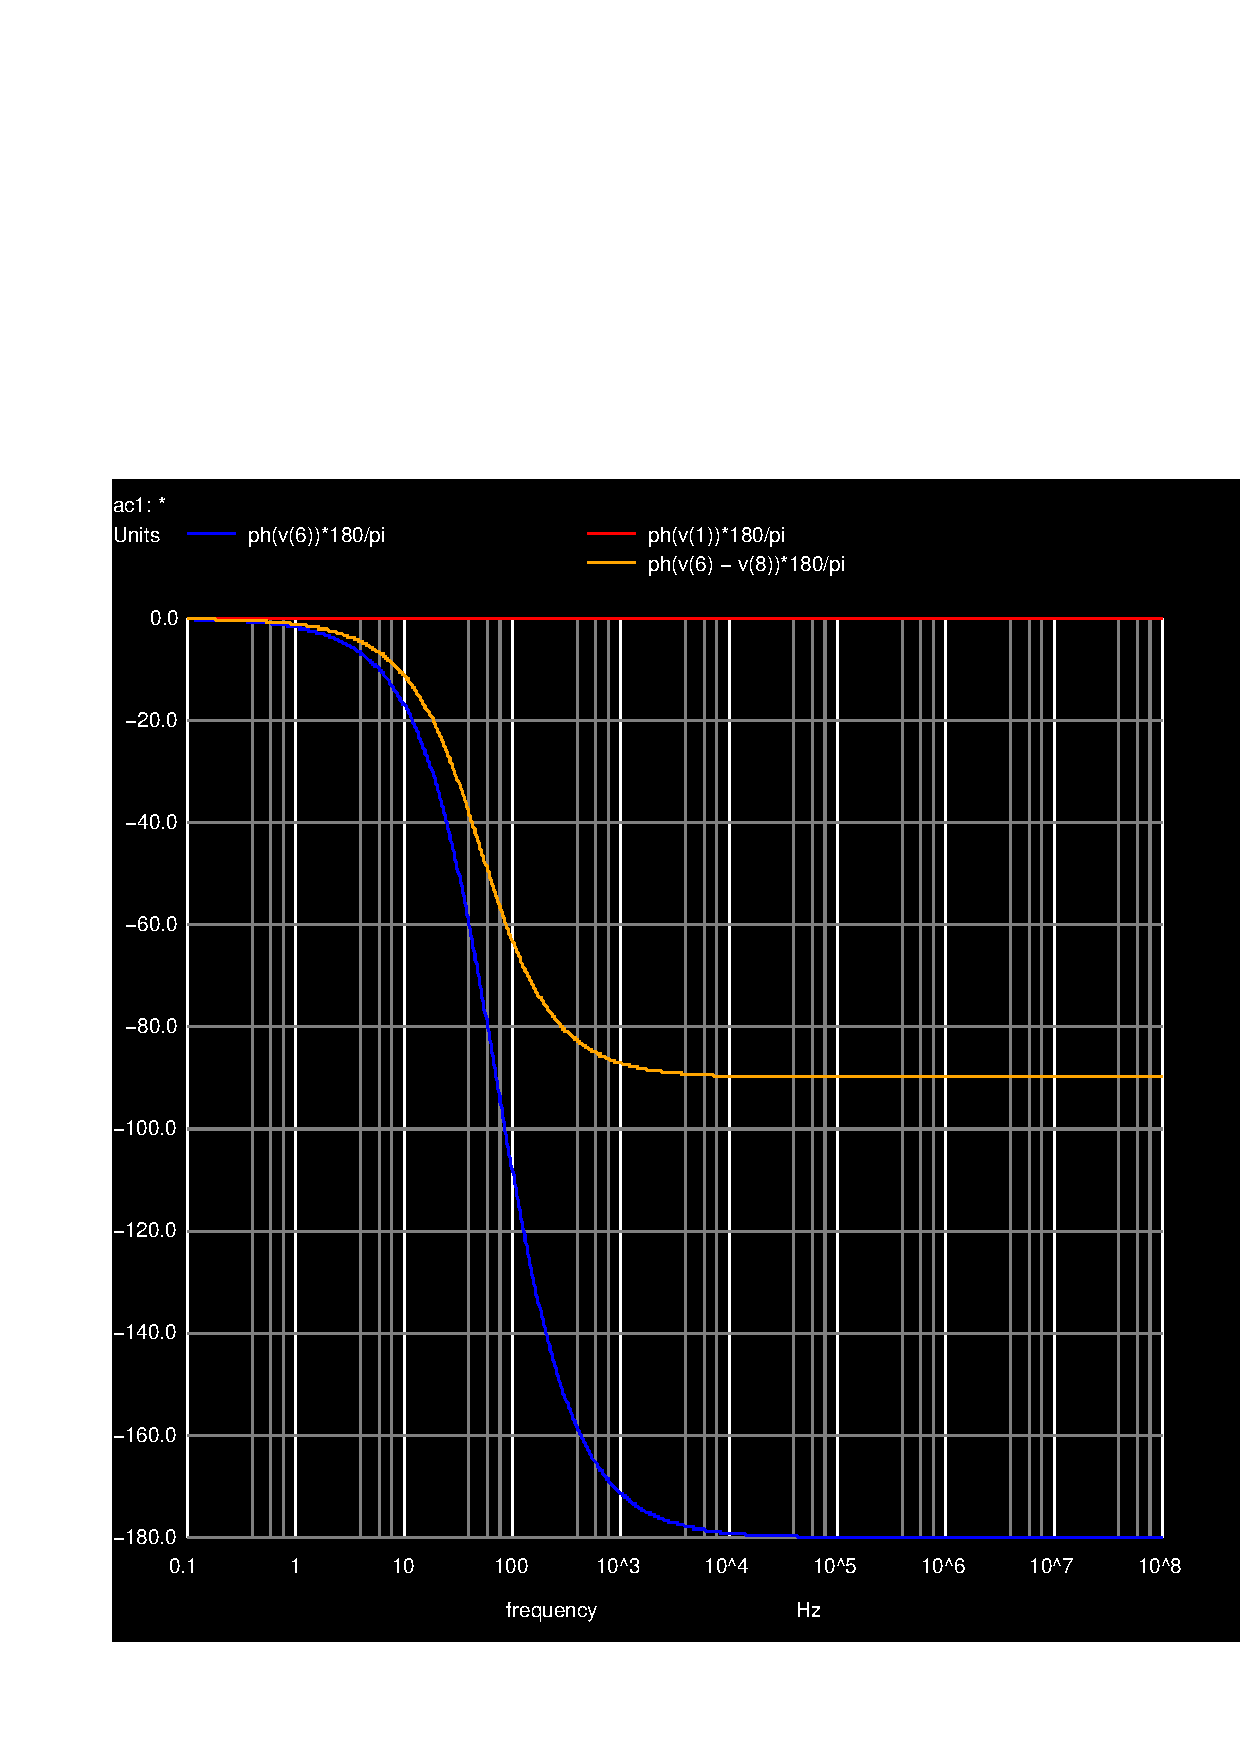
\includegraphics[width = 15cm]{sim5_ph.pdf}
%\caption {Ngspice simulation plot 4}
%\end{figure}

